\section{Data Collection Study}
We conducted a data collection study to gather IMU data while performing touches on a smartphone.
Our collected data set consists of 6 smartphone sensors that were sampled while participants performed successive touches on the smartphones front side. 
%Here report: How and why is the data collection study designed as it is?
\subsection{Design}
We used a repeated-measures design with one independent variable: \textsc{phone}, which was counterbalanced using Latin Balanced squares. To total amount of conditions was: \textsc{phone} $ = 4$.
\subsection{Apparatus}

Our dataset was generated using four different sized smartphones on which participants had to perform a certain amount of touches (for further information see \cref{sec:tasks}).
Our used phone sizes range from $ 4^{\prime\prime} $ (S3) to $ 6^{\prime\prime} $ (N6). 
Using phones of these sizes we were able to cover the sizes of everyday smartphones, including some high-end devices and create a generalizable machine-learning model.
For more technical details about the used devices see \cref{tab:devices}.
\begin{table}[t]
	\centering
	\begin{tabularx}{1\textwidth}{Xcd{3.1}d{2.2}d{1.2}d{2.2}d{1.2}d{1.2}}%{Xrd{1.2}d{3.1}d{2.2}d{1.2}d{2.2}d{1.2}d{1.2}}
		\toprule
		\multicolumn{1}{l}{\multirow{3}{*}{\shortstack[c]{\textbf{Device}}}}&
		\multicolumn{1}{c}{\multirow{3}{*}{\shortstack[c]{\textbf{Release}}}}&    
		\multicolumn{1}{c}{\multirow{3}{*}{\shortstack[c]{\textbf{Weight}\\ \textbf{(g)}}}} &
		\multicolumn{1}{c}{\multirow{3}{*}{\shortstack[c]{\textbf{Screen}\\ \textbf{Diagonal}\\ \textbf{(in)}}}} &
		\multicolumn{1}{c}{\multirow{3}{*}{\shortstack[c]{\textbf{Height}\\ \textbf{(cm)}}}} &
		\multicolumn{1}{c}{\multirow{3}{*}{\shortstack[c]{\textbf{Width}\\ \textbf{(cm)}}}} &
		\multicolumn{1}{c}{\multirow{3}{*}{\shortstack[c]{\textbf{Depth}}}} \\ 
		\\
		\\
		\midrule
		%                        year  weight diag  height  width  depth
		Samsung Galaxy S3 Mini  & 2012 & 113 &  4. & 12.16 & 6.3  & 0.99 \\
		Samsung Galaxy S4 		& 2013 & 130 &5.   & 13.7  & 7.0  & 0.79 \\
		Google Nexus 5X 		& 2015 & 136 &5.2 & 14.7  & 7.26 & 0.79 \\
		Motorola Nexus 6 		& 2014 & 184 & 6.  & 15.93 & 8.3  & 1.01 \\ 
		\bottomrule
	\end{tabularx}%
	\caption[Smartphone data]{\small Data about the smartphones that were used in the study.}
	\label{tab:devices}
\end{table}

\subsection{Tasks}
\label{sec:tasks}

\begin{marginfigure}
	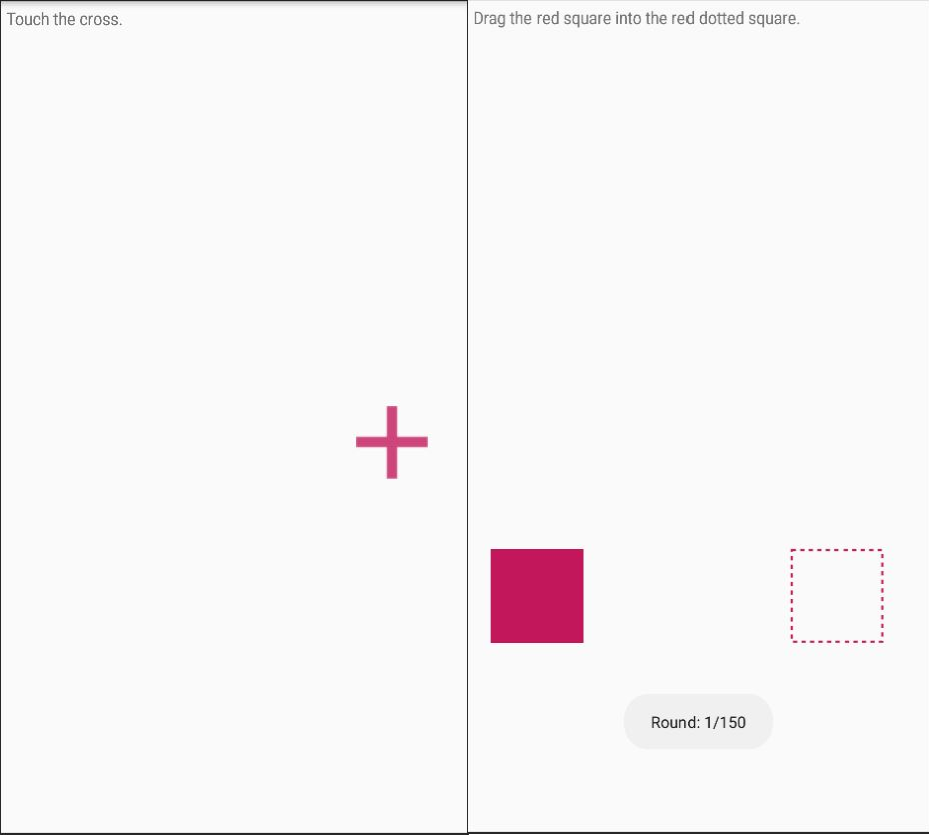
\includegraphics[width=\marginparwidth]{scur}
	\caption{SCUR.}
	\label{fig:tasks}
\end{marginfigure}


For our data collection study participants had to perform a series of touches on the smartphones' touchscreen. 
We aligned the touch points displayed as crosses in a 16 $ \times $ 9 grid. 
In order to achieve a high variance across the whole screen, we randomized the positions of the crosses within all the cells.
To avoid sequential effects, we randomized the order in which the crosses were displayed.
There were a total of 3 repetitions, resulting in a total  of $ 16 \times 9 \times 3 = 432 $ touches on one device.

Between two touches our study participants had to perform a simple \textit{Fitts' Law task}. 
Here participants had to drag a filled rectangle into a dashed contour of a rectangle.
This task was mainly implemented to reset the participants grip to the bottom half of the device.
Because a previous shifted grip of the hand to the upper half of the phone influences the recorded sensor data when reaching for the next target in the lower half and vice versa. 
See \cref{fig:tasks} for a more detailed view of the tasks.
\subsection{Procedure}
Participants were either invited within the course \textit{FIS'18}.
All appointments were discussed orally.
After participants have arrived they signed a consent form. 
We then continued measuring their hand length.
We asked the participants to take a seat on a chair without armrests and explained the study procedure and its sense.
We started carrying out the study and handed out the first phone accordingly to the balanced Latin Square order. 
After participants finished the tasks (see \cref{sec:tasks}) on the first phone, we asked them if they need a short recovery break and then continued with the next phones.
Additionally, we allowed participants to rest and put away the phone during the \textit{Fitt's Law task} because we specifically deal with this task in our preprocessing step (see \cref{sec:prepro}).
The study duration was \textbf{X} minutes on average.
\subsection{Participants}
%Some sentences are copied from Beens BA, is this sufficient? ASK SVEN OR HUY
\textbf{UPDATE ON STUDY FINISH}

We invited 20 participants (14 male, 4 female).
Their age ranged between 21 and 27 ($ M=24.28$ , $SD=1.67 $). 
All participants were fellow students. 
We only invited right-handed people.
We measured the hand length of participants. 
The size was measured from the tip of the middle finger to the wrist crease with fingers stretched out.
Hand lengths ranged from $16.0cm$ to $21.3cm$ ($M=19.44cm$ , $SD=1.4cm$).
Our measured data covers samples from the 5th and 95th percentile of the anthropometric data reported in previous work \cite{Poston}.  
